\documentclass{school-22.211-notes}
\date{May 23, 2012}

\begin{document}
\maketitle

%%%%%%%%%%%%%%%%%%%%%%%%% Qualify Exam Start %%%%%%%%%%%%%%%%%%%%%%%%%%%%
\lecture{Qualify Exam Recap}
%Kord mentioned 09/10/12 that Prompt jump approximation is a classical qual problem.

\topic{Basics (with questions)}
\begin{enumerate}
\item Common units, see Table~\ref{units}. Angular flux is scalar quantity and the term with angular dependency is $n$ not $v$. 
\begin{table}[ht]
  \centering
  \begin{tabular}{|c|c|c|c|c|c|} \hline
   $\sigma$ & $\Sigma$ & $\phi = nv$  & $J$ & $R = \phi \Sigma$ & RI  \\ \hline
   $\cm^2$ & $1/\cm$ & $\frac{n}{\cm^2 \s}$  & $\hat{e} \frac{n}{\cm^2 \s}$ & $\frac{\mathrm{reactions}}{\cm^3 \s}$ & barns \\ \hline
  \end{tabular}
  \caption{Units of Common Terms} \label{units}
\end{table}
\item 1 GWd/MT = 30 days = 30 million dollars. 
\item Boron worth: -16 pcm/ppm. Approximate as -10 pcm/ppm. 
\item PWRs have 20\% $\Delta k$ reactivity hold-down, whereas BWRs only have 2\% (b/c the use of Gd; Gd behaves like onion skin burning; Gd can control burning by density). 
\item Fast flux in hydrogen is around $10^{14}$ n/cm$^2$s, and on the order of $10^{12}$n/cm$^2$s for thermal flux. 
\item Average energies prompt neutrons are released: 2 MeV (peak prompt neutron energies: 0.7 MeV). Average energies delayed neutrons are released: 0.4 MeV. 
\item Core decay heat after 1 day is about 1\% rated. 
\item Constants to know: 1u = 931.5 MeV. 
\item The effect of U238 energy self-shielding is about an effect of 10, that is, going from infinite dilution to U/I = 0.1. 

\item Reactivity units. 
\begin{table}[ht]
  \centering
  \begin{tabular}{|c|c|c|} \hline
    Unit & Definition & Example \\ \hline
    $\Delta k$ & actual units of PKEs & 0.01 \\
    \% $\Delta k$ & & 1\% \\
    pcm & $10^5 \Delta k $ & 1000 pcm \\ \hline
    Dollars & $\frac{\Delta k}{\beta}$ & \$1.5 \\
    Cents & 100 Dollars & 150 cents \\ 
    Milli-beta & 1000 Dollars & 1500 milli-beta \\ \hline
  \end{tabular}
\end{table}
\end{enumerate}


\textbf{General Knowledge Practice Questions}
\begin{enumerate}
\item (Qual 2012). 
\begin{enumerate}
\begin{figure}[ht]
  \centering
  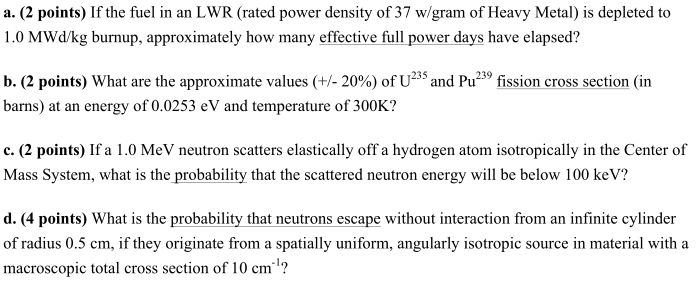
\includegraphics[width=6in]{images/qual/general_knowledge.png}
\end{figure}
\item We approximate 1 GWd/MT (that is 1 MWd/kg) as 30 days of operation. 

\item Fission cross section at 0.1eV and 300K for \ce{U^{235}} is 250b, for \ce{Pu^{239}} is about 475b. 

\item The pdf is a flat distribution, so it is equally likely to get anywhere below 1.0 MeV, then the change of below 100 keV is 100 keV/1 MeV = 10\%. 

\item We treat this as a fuel to moderator two-region problem. Then we can calculate fuel to fuel probability. First we calculate chord length $l = \frac{4V}{S} = \frac{4 \pi r^2 H}{2 \pi r H} = 2r = 1\fsp \cm.$
\eqn{ P_{FF} = \frac{\Sigma_t^F (u)}{\Sigma_t^F (u) + \Sigma_e}  = \frac{10}{10 + 1} = 0.909 } 
Thus the probability of escaping the cylinder is just 9.09\%. 

\end{enumerate}
\end{enumerate}


\clearpage
\topic{Cross Section}
\begin{enumerate}
\item* If the neutron cross section is independent of energy at 0K, at 1200K the cross section would have a 1/v energy shape because of thermal motion. 
  
\item* Resonance absorption cross section dominates resonance scattering cross section most of the time (except U238). 

\item* Fission cross section: U235 fission xs at 0.1 eV and 300K is about 200 barns (200-300 barns); Pu239 fission xs is about 475 barns (380-570 barns). Hence in thermal reactors, Pu absorption should be about twice that of uranium. 

\item Elastic scattering cross section as in Figure~\ref{scatter-xs}
\begin{figure}
  \centering
  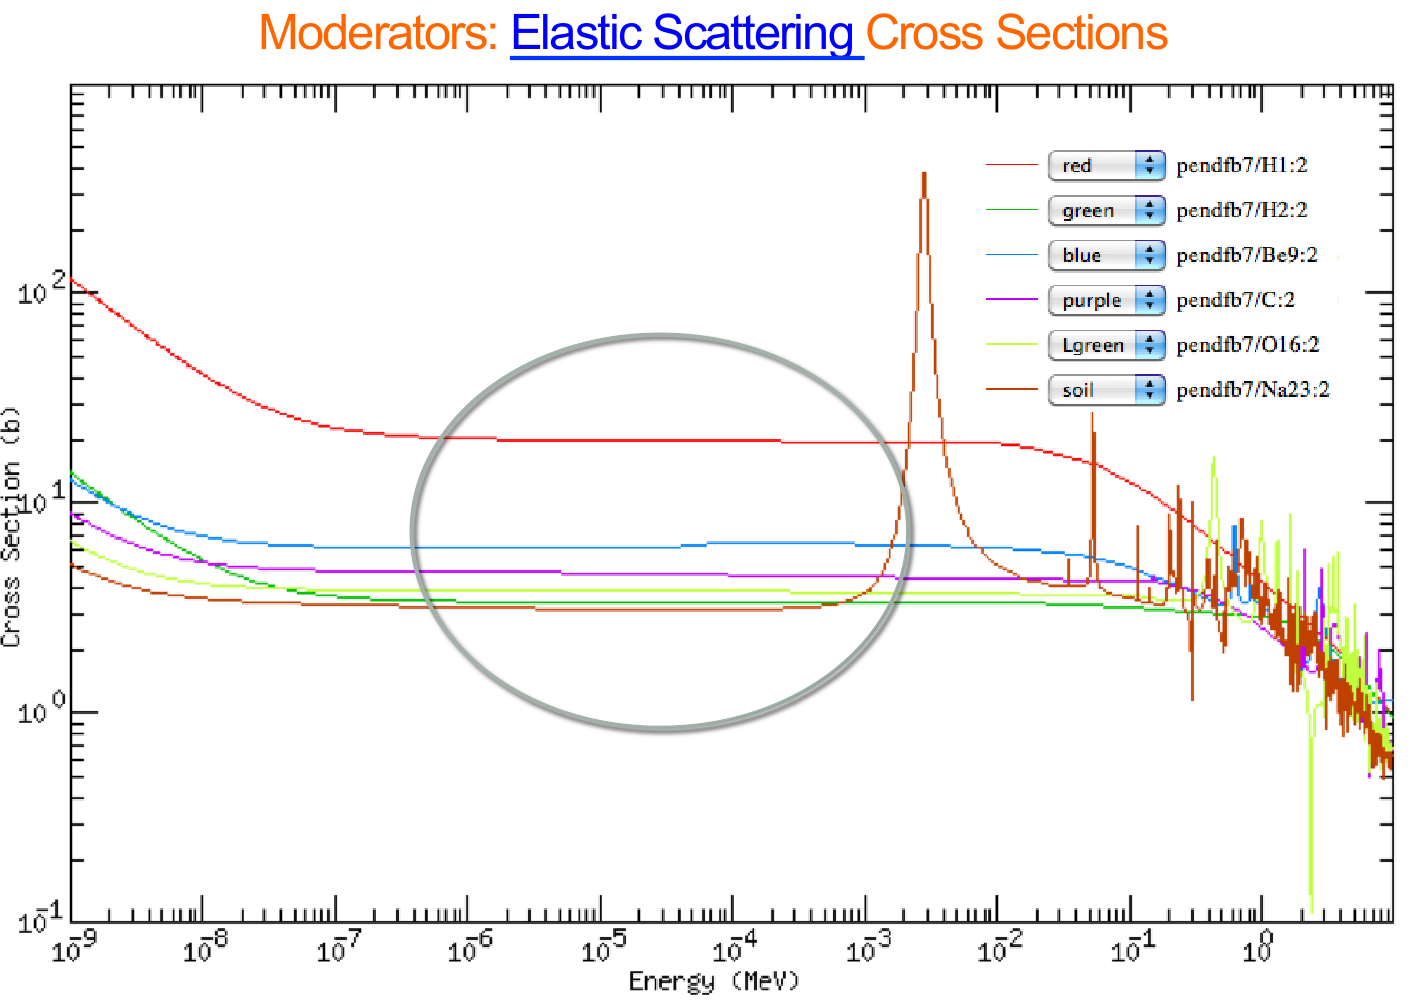
\includegraphics[width=6in]{images/intro/scatter-xs-moderator.png}
  \\
  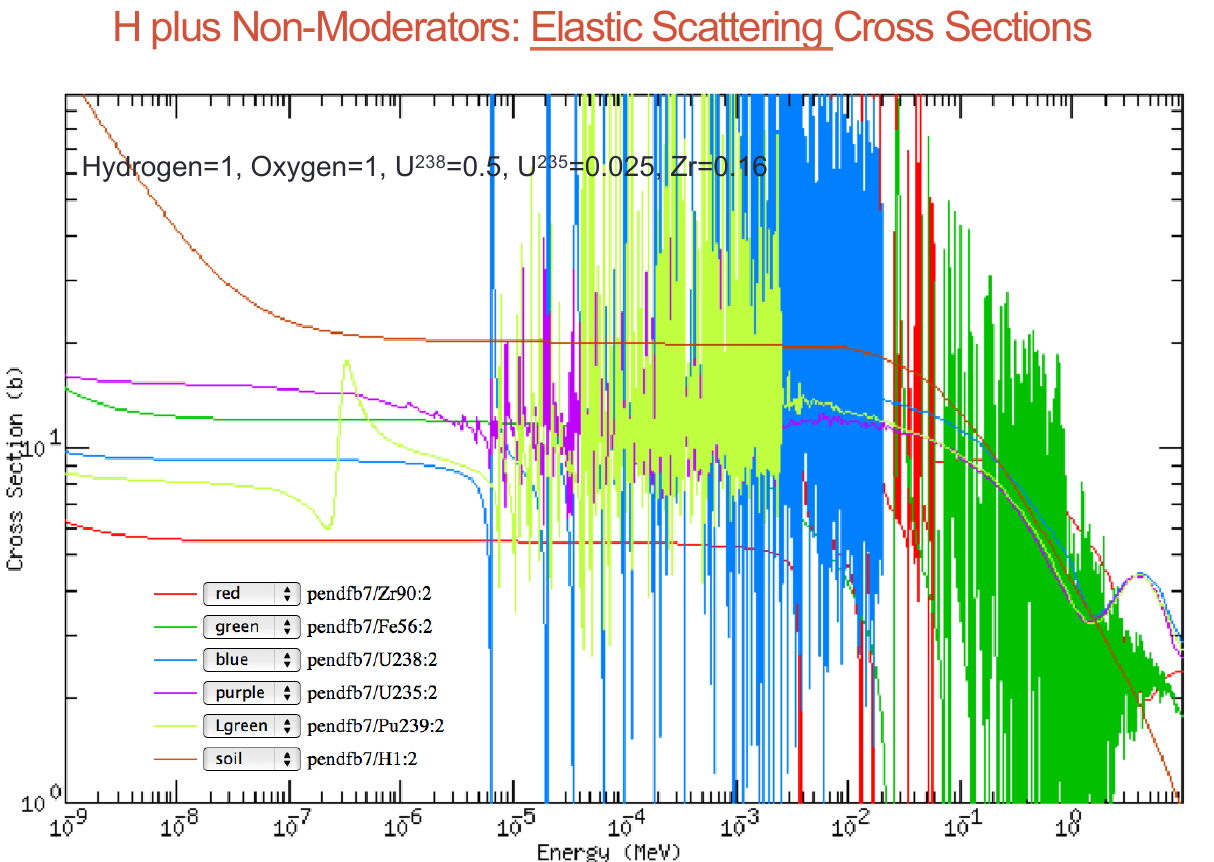
\includegraphics[width=6in]{images/intro/scatter-xs-LWR.png}
  \caption{Elastic Scattering Cross Sections} \label{scatter-xs}
\end{figure}

\item Capture cross section as in Figure~\ref{capture-xs}: 
  \begin{figure}
    \centering
    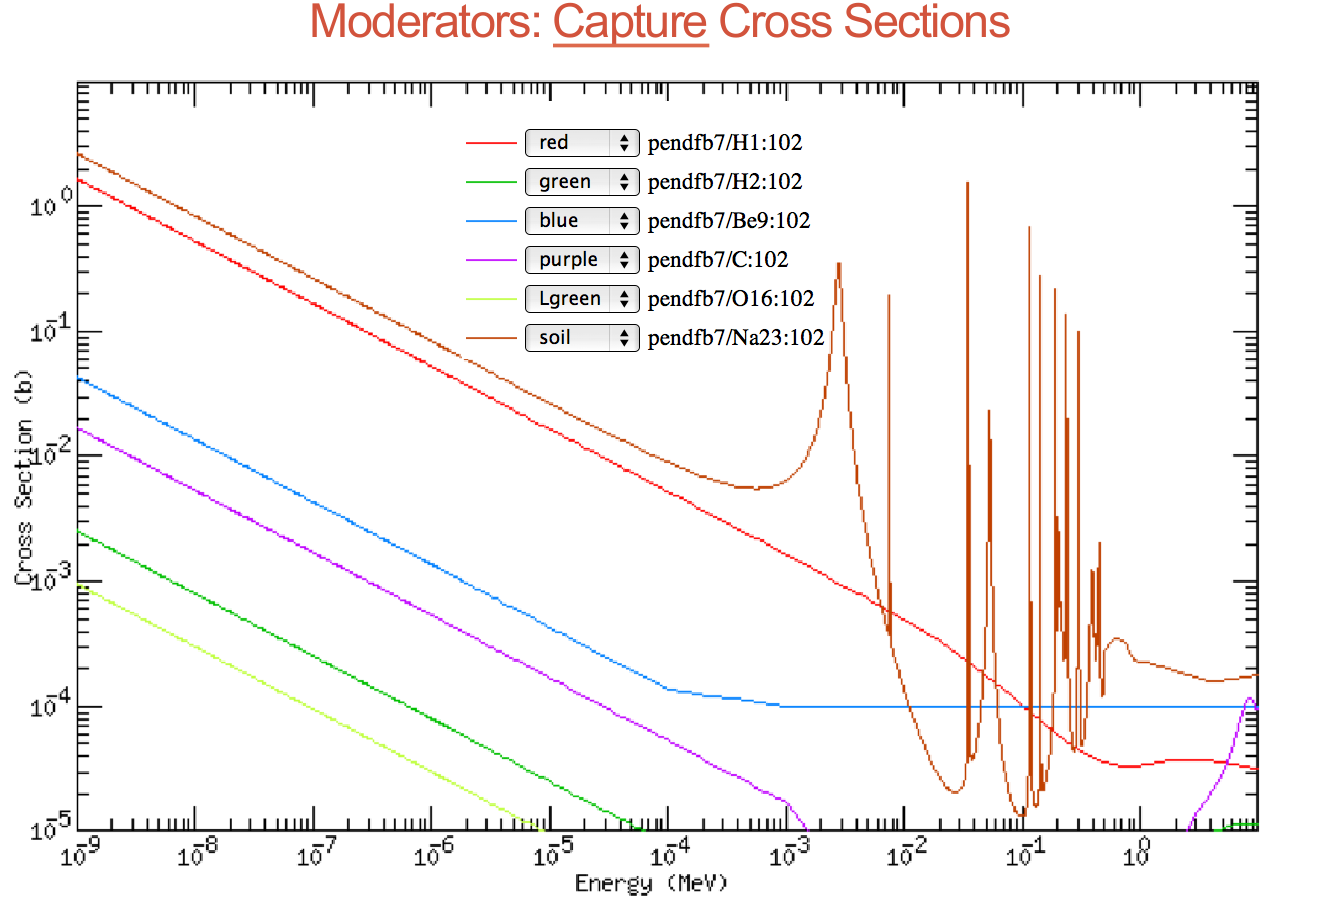
\includegraphics[width=6in]{images/intro/capture-xs.png}
    \\
    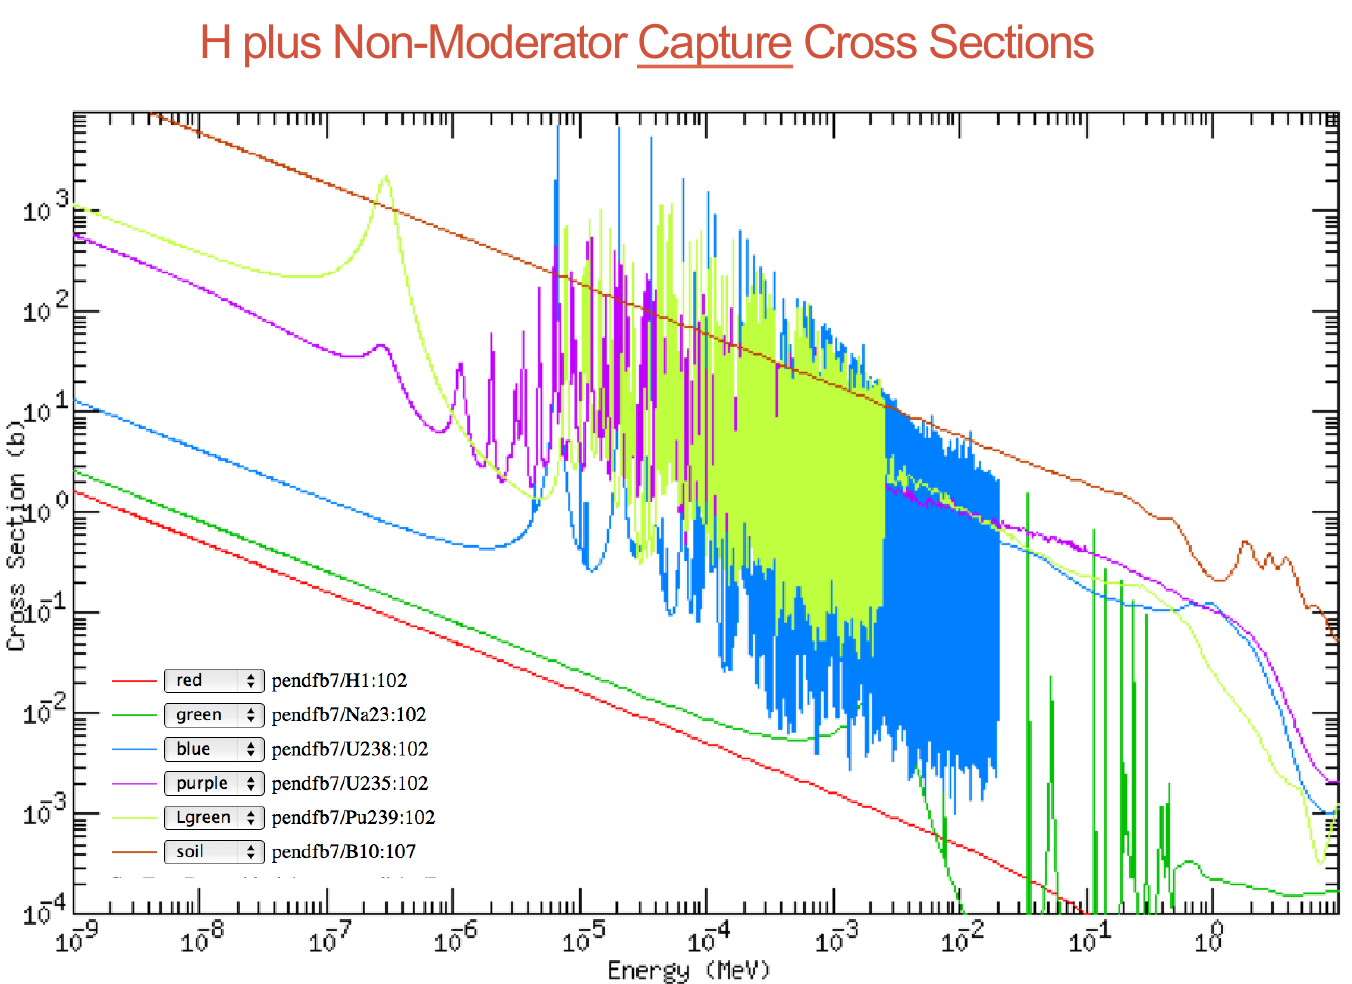
\includegraphics[width=6in]{images/intro/capture-xs-2.png}
    \caption{Capture Cross Section} \label{capture-xs}
  \end{figure}
  \begin{enumerate}
  \item H has no resonance; it has the highest scattering xs in LWR, so we can ignore any other isotopic's neutron scattering.   
  \item Na has a huge resonance in 23 keV, and more resonances at higher energies because it is a heavy isotope.
  \item Near zero energy,
    \eqn{ \sigma(E\to 0) \propto \sqrt{\frac{kT}{AE}}    }
  \item Resonance at 6 to 7 eV: U238. 
  \item U235's thermal elastic xs is larger than 238's, and they both have resonance around the same range.   
  \item A small resonance at .3 eV: Pu239 (its signiture is a super low energy scattering xs). 
  \end{enumerate}

\item Given an unknown material type, all we care is to count the nucleus density of each material and look at it's xs. 
\end{enumerate}


\clearpage
\topic{Steady State} 
\begin{enumerate}
\item A PWR typically have a Doppler coefficient of -3 pcm/K. 

\item One Group $\kinf$: in one group $k_{\infty}$ only depends on cross sections $k_{\infty} = \frac{\nu \Sigma_f}{\Sigma_a}$ and has no flux dependency. The flux is buried in the calculation of cross section.

\item Two group $\kinf$: we start with neutron balance equation:
  \begin{align}
    \frac{\nu \Sigma_{f1}}{k_{\infty}} \Phi_1 - \Sigma_{a1} \Phi_1 - \Sigma_{s12} \Phi_1 + \frac{\nu \Sigma_{f2}}{k_{\infty}} \Phi_2 + \Sigma_{s21} \Phi_2 &= 0 \\
\Sigma_{s12} \Phi_1 - \Sigma_{s21} \Phi_2 - \Sigma_{a2} \Phi_2 &= 0 
  \end{align}
  Typically what we do is to write it in a matrix form and solve for a coupled system. But even better, we can define the \hi{effective removal rate} $\bar{\Sigma}_{s12}$, and re-write the two-group balance equation: 
  \begin{align}
    \frac{\nu \Sigma_{f1}}{k_{\infty}} \Phi_1 - \Sigma_{a1} \Phi_1 - \bar{\Sigma}_{s12} \Phi_1 + \frac{\nu \Sigma_{f2}}{k_{\infty}} \Phi_2 &= 0 \\
    \bar{\Sigma}_{s12} \Phi_1- \Sigma_{a2} \Phi_2 &= 0 
  \end{align}
  Then we can solve for $\frac{\Phi_1}{\Phi_2}$ from the second equation in terms of cross section, plug in the first equation, and get $k_{\infty}$ from there. Notice that we only know the relative magnitude of $\Phi$ and $\Phi_2$. 

\item Know Two-group diffusion model: group 1 is the fast group larger than 0.625 eV, and group 2 is the thermal group. 
\begin{enumerate}
\item $D_1 = 1.5, D_2 = 0.5$.
\item Total fission source: $\chi_1 = 1.0, \chi_2 = 0.0$ implies that the fission source in thermal group is zero,
  \eqn{ S_f(\vecr) = \chi_g \Sum_g \nu \Sigma_{fg} (\vecr) \phi_g(\vecr) }
\item Scattering source: define effective down-scatter, so up-scattering is zero $\Sigma_{s21} (\vecr) = 0$. 
\item Final Two-Group Diffusion Equations: 
  \eqn{\boxed{ -\divergence D_1 \gradient \phi_1 + [\Sigma_{a1} + \Sigma_{s12} ] \phi_1 = \nu \Sigma_{f1} \phi_1 + \nu \Sigma_{f2} \phi_2 + S_1} }
  \eqn{\boxed{ -\divergence D_2 \gradient \phi_2 + \Sigma_{a2} \phi_2 = \Sigma_{s12} \phi_1 + S_2} }
\end{enumerate}

\item Know the one-group fundamental mode eigenvalues and eigenvectors as in Table~\ref{eigen-values}. 
\begin{table}[ht]
  \centering
  \begin{tabular}{|l|l|l|} \hline
     Slab $\in  \left[- \frac{L}{2}, \frac{L}{2} \right]$ & $\phi(x) = A \cos \left( \frac{\pi x}{L} \right)$ & $B^2 = \left( \frac{\pi}{L} \right)^2$ \\ \hline
     Sphere $\in [0, R]$ & $\phi(r)= A\frac{\sin \left( \frac{\pi r}{R} \right)}{r} $ & $B^2 = \left( \frac{\pi}{R} \right)^2$ \\ \hline
     Infinite cylinder $\in [0, R]$ & $\phi(r) = A J_0 \left( \frac{2.405 r}{R} \right)$ & $B^2 = \left( \frac{2.405}{R} \right)^2$ \\ \hline
     Finite cylinder $r \in [0, R], z \in \left[ -\frac{H}{2}, \frac{H}{2} \right]$ & $\phi(r,z) = A J_0\left( \frac{2.405 r}{R} \right) \cos \left( \frac{\pi z}{H} \right)$ & $B^2 = \left( \frac{2.405}{R} \right)^2 + \left( \frac{\pi}{H} \right)^2$ \\ \hline
     Parallelepiped $\in \left[ -\frac{L_i}{2}, \frac{L_i}{2} \right]$ & $\phi(x) = A \cos \left( \frac{\pi x}{L_x} \right) \cos \left( \frac{\pi y}{L_y} \right) \cos \left( \frac{\pi x}{L_z} \right)$ & $B^2 = \left( \frac{\pi}{L_x} \right)^2 + \left( \frac{\pi}{L_y} \right)^2 + \left( \frac{\pi}{L_z} \right)^2$ \\ \hline
  \end{tabular}
\end{table}

\end{enumerate}




\clearpage
\topic{Kinetics}








\end{document}
